\documentclass[letterpaper,11pt]{article}

\usepackage{latexsym}
\usepackage[empty]{fullpage}
\usepackage{titlesec}
\usepackage{marvosym}
\usepackage[usenames,dvipsnames]{color}
\usepackage{verbatim}
\usepackage{enumitem}
\usepackage[hidelinks]{hyperref}
\usepackage{fancyhdr}
\usepackage[english]{babel}
\usepackage{tabularx}
\usepackage{fontawesome5}
\usepackage{multicol}
\setlength{\multicolsep}{-3.0pt}
\setlength{\columnsep}{-1pt}
\input{glyphtounicode}

%new packages

\usepackage{fontenc}
\usepackage{amsmath}
\usepackage{amssymb}
\usepackage{graphicx}



%----------FONT OPTIONS----------

\pagestyle{fancy}
\fancyhf{} % clear all header and footer fields
\fancyfoot{}
\renewcommand{\headrulewidth}{0pt}
\renewcommand{\footrulewidth}{0pt}

% Adjust margins
\addtolength{\oddsidemargin}{-0.6in}
\addtolength{\evensidemargin}{-0.5in}
\addtolength{\textwidth}{1.19in}
\addtolength{\topmargin}{-.7in}
\addtolength{\textheight}{1.4in}

\urlstyle{same}

\raggedbottom
\raggedright
\setlength{\tabcolsep}{0in}

% Sections formatting
\titleformat{\section}{
  \vspace{-4pt}\scshape\raggedright\large\bfseries
}{}{0em}{}[\color{black}\titlerule \vspace{-5pt}]



% Ensure that generate pdf is machine readable/ATS parsable
\pdfgentounicode=1

%-------------------------
% Custom commands
\newcommand{\resumeItem}[1]{
  \item\small{
    {#1 \vspace{-2pt}}
  }
}

\newcommand{\classesList}[4]{
    \item\small{
        {#1 #2 #3 #4 \vspace{-2pt}}
  }
}

\newcommand{\resumeSubheading}[4]{
  \vspace{-2pt}\item
    \begin{tabular*}{1.0\textwidth}[t]{l@{\extracolsep{\fill}}r}
      \textbf{#1} & \textbf{\small #2} \\
      \textit{\small#3} & \textit{\small #4} \\
    \end{tabular*}\vspace{-7pt}
}

\newcommand{\resumeSubSubheading}[2]{
    \item
    \begin{tabular*}{0.97\textwidth}{l@{\extracolsep{\fill}}r}
      \textit{\small#1} & \textit{\small #2} \\
    \end{tabular*}\vspace{-7pt}
}

\newcommand{\resumeProjectHeading}[2]{
    \item
    \begin{tabular*}{1.001\textwidth}{l@{\extracolsep{\fill}}r}
      \small#1 & \textbf{\small #2}\\
    \end{tabular*}\vspace{-7pt}
}


\newcommand{\resumeSubItem}[1]{\resumeItem{#1}\vspace{-4pt}}

\renewcommand\labelitemi{$\vcenter{\hbox{\tiny$\bullet$}}$}
\renewcommand\labelitemii{$\vcenter{\hbox{\tiny$\bullet$}}$}

\newcommand{\resumeSubHeadingListStart}{\begin{itemize}[leftmargin=0.0in, label={}]}
\newcommand{\resumeSubHeadingListEnd}{\end{itemize}}
\newcommand{\resumeItemListStart}{\begin{itemize}}
\newcommand{\resumeItemListEnd}{\end{itemize}\vspace{-5pt}}

\begin{document}
\fontfamily{cmr}\selectfont
\begin{center}
\parbox{3.0cm}{%
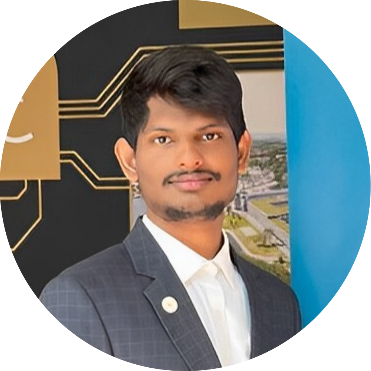
\includegraphics[width=2.7cm,clip]{images/resume_pic_m.png}}
}
\parbox{\dimexpr\linewidth-3.8cm\relax}{
\vspace{-20pt}
\begin{tabularx}{\linewidth}{L r} \\
    {\Huge \scshape  Venkata Sai Yakkshit Reddy Asodi}~
    \href{https://www.cedzlabs.com/yakkshit}{\vspace{1pt}}\\
      Berlin, Germany. \\ \vspace{1pt}
     \small \raisebox{-0.1\height}\faPhone\ +91 8179936156 ~ \href{mailto:saiyakkshit2001@gmail.com}{\raisebox{-0.2\height}\faEnvelope\  {saiyakkshit2001@gmail.com}} ~ 
    \href{https://linkedin.com/in/yakkshit/}{\raisebox{-0.2\height}\faLinkedin\ {yakkshit}}  ~
    \href{https://yakkshit.com/}{\raisebox{-0.2\height}\faGlobe\ {yakkshit.com}}  ~
    \href{https://github.com/yakkshit}{\raisebox{-0.2\height}\faGithub{ yakkshit}}
    \vspace{-8pt}
    
\end{tabularx}
}
\end{center}

\vspace{-23pt}
%-----------EDUCATION-----------
\href{https://www.yakkshit.com/#details}{\section{Summary \faLink}
Aspiring Full Stack Developer with a strong foundation in frontend and backend technologies. Adept at problem-solving and eager to learn new skills. Proven experience in developing responsive applications and collaborating in team environments. Passionate about creating efficient and user-friendly software solutions.}

%-----------PROGRAMMING SKILLS-----------
\section{\href{https://www.linkedin.com/in/yakkshit/details/skills/}{Technical Skills} \faLink}
\begin{itemize}[leftmargin=0.15in, label={}]
\small{\item{
\textbf{Frameworks - }{React, Node.js, Express, Bootstrap, Figma.} \\
\textbf{Languages - }{JavaScript (ES6+), HTML5, CSS3, PHP, Python.} \\
\textbf{Tools - }{Git, Docker, Postman, Swagger, RESTful APIs.} \\
\textbf{Deployment - }{AWS, Azure, Nginx.}\\
}}
\end{itemize}
\vspace{-10pt}

%-----------EXPERIENCE-----------
\section{Experience \faLinkedin}

\resumeSubHeadingListStart

\resumeSubheading
{\large Circleup AG \faBuilding}{December 2023 -- July 2024}
  {Lead Full Stack Engineer (Frontend Focus)}{\faMapMarker \hspace{0.1cm} Zurich, Switzerland}\\
\vspace{10pt}
\textbf{Responsibilities:}
\resumeItemListStart
\vspace{-10pt}
\resumeItem{Developed responsive web applications using the Meteor framework, ensuring seamless user experiences for AI-driven services. Collaborated closely with backend developers to integrate APIs, focusing on LLM-TGI-related endpoints.}
\resumeItem{Led the design and implementation of modern, user-centered UI/UX, creating reusable components and maintaining a design system. Optimized applications for scalability and performance in a fast-paced startup environment.}
\resumeItemListEnd
\vspace{-3pt}
\textbf{Environment:}\emph{Meteor, React, Figma, JavaScript, RESTful APIs, Agile methodologies.}

\resumeSubheading
{Cedzlabs \faBuilding}{March 2023 -- July 2024}
{Full Stack Developer}{\faMapMarker \hspace{0.1cm} India.}\\
\vspace{10pt}
\textbf{Responsibilities:}
\vspace{-10pt}
\resumeItemListStart
\resumeItem{Created intuitive UI/UX designs for web applications, focusing on responsive and accessible design principles. Collaborated with cross-functional teams to gather requirements and deliver projects on time.}
\resumeItemListEnd
\vspace{-3pt}
\textbf{Environment:}\emph{React, CSS3, HTML5, Figma, Git.}

\resumeItem{\textbf{\href{https://linkedin.com/in/yakkshit}{Checkout my other experiences by clicking here}}}
\vspace{-5pt}

%-----------PROJECTS-----------
\section{Projects \faGithub}
\vspace{-5pt}
\resumeSubHeadingListStart
\resumeProjectHeading
{\textbf{\href{https://ui.cedzlabs.com/resume}{AI Resume Tuner}} $|$ \emph{Azure Cloud, Next.js, RAG, LLMs}}{August 2023 $|$ \faBuilding \hspace{0.1cm}Microsoft}\\
\vspace{6pt}
\textbf{Description:}
\vspace{-5pt}
\resumeItemListStart
\resumeItem{Developed an AI-powered resume tuner that takes candidate details and job descriptions as inputs to generate customized resumes. The project, built using Retrieval Augmented Generation (RAG) and multimodal LLMs, was part of a Microsoft Hackathon. Integrated the backend APIs with a Next.js frontend to create a user-friendly interface for designing tailored resumes. The backend was deployed on Azure Cloud to ensure scalability, secure data handling, and fast performance.}
\resumeItemListEnd
\vspace{4pt}
\textbf{Tools:}\emph{
Next.js, Azure Cloud, RAG, LLMs, Microsoft AI Studio.}
\vspace{-10pt}

\resumeProjectHeading
{\href{https://yakkshit.com}{\textbf{Portfolio Website}} $|$ \emph{NextJS, AWS}}{January 2023}\\
\vspace{6pt}
\textbf{Description:}
\vspace{-5pt}
\resumeItemListStart
\resumeItem{Designed and implemented a secure file encryption/decryption system on AWS, built and deployed a scalable website using NextJS, and created a user-friendly UI/UX for my portfolio using Figma and React.}
\resumeItemListEnd
\vspace{4pt}
\textbf{Tools:}\emph{NextJS, AWS, Figma, React.}
\vspace{-12pt}

\section{Languages}
\begin{itemize}
  \item Telugu - Native $|$ English - Fluent $|$ Hindi - Fluent $|$ German - Elementary $|$ Swedish - Elementary.
\end{itemize}

%-----------INVOLVEMENT---------------
\section{Achievements / Extracurricular / Contributions}
\resumeSubHeadingListStart
\resumeItemListStart
\resumeItem{Experience implementing Agile methodologies, including Scrum and Kanban.}
\resumeItem{Contributed to various open-source projects related to web development and design systems.}
\resumeItem{Active participant in tech meetups and workshops, focusing on UI/UX best practices.}
\resumeItemListEnd

\resumeSubHeadingListEnd
\textbf{Strengths : }\emph{Leadership, self-motivation, attention to detail, and adaptability.} \\

\vspace{10pt}
\end{document}